\chapter{Decisiones y soluciones}

Una vez están claros los requisitos y se les ha realizado un análisis para su posterior implementación, podemos empezar a comentar las decisiones tomadas y las soluciones implementadas.\\

Pero antes, cabe decir que el principal motivo que me animó a adentrarme en este proyecto fue mi experiencia con muchas distribuciones basadas en \textit{GNU/Linux} adquirida a lo largo de la carrera. Siempre me ha gustado instalarlas en mi ordenador para probarlas, luego desinstalarlas y pasar a probar otras nuevas. Pasar por eso me ha obligado a lidiar con gestores de arranque, administradores de paquetes, configuraciones de sistemas de ficheros y entornos de escritorio, entre otras cosas.\\

Gracias a esto, he podido ver con soltura y abstracción las diferentes piezas de este puzzle llamado \textit{``Meta-DYNAsystem''}, aplicando mis conocimientos previos para desarrollar un sistema lo más robusto posible.\\

Ya venimos hablando largo y tendido sobre dispositivos embebidos, pero es ahora cuando hablaremos de las alternativas elegidas para infraestructura física y virtual, las herramientas de desarrollo de la distribución, y por último del gestor de actualizaciones.

\section{Infraestructura física elegida}

Como anticipábamos en el estado del arte, existen diferentes posibilidades en un proyecto a la hora de desarrollar una infraestructura física que abastezca a un sistema informático:\\

-- Por ejemplo, podríamos optar por montar un ordenador de sobremesa de formato convencional e instalar ahí la infraestructura virtual; dotándola de unas mayores capacidades computacionales, a expensas del precio.\\

-- O por otro lado, encontramos la opción de utilizar un computador \textit{SBC} de los ya mencionados; lo que ajustaría mucho el precio de coste disminuyendo también la potencia máxima del sistema.\\

Para empezar, como comentamos en la descripción del problema, la empresa tenía como premisa reducir los precios de coste del producto original, que llevaba instalado un ordenador convencional en formato \textbf{\textit{Mini-ITX}}.

\begin{quotation}
	\textit{Mini-ITX} es un formato de placa base para ordenadores compactos. Fue desarrollado de forma propietaria por la compañía \textit{VIA Technologies}, desencadenó un gran uso de este formato y posteriormente sus especificaciones pasaron a ser libres \cite{via-mini-itx}.
\end{quotation}

Por una parte, el computador integrado en la máquina antigua disponía de una buena escalabilidad, dado que poseía unas buenas prestaciones. Sin embargo, dichas prestaciones \textbf{no eran necesarias}. Para un sistema dedicado con una sola aplicación embebida, podía utilizarse un ordenador más ajustado tanto en rendimiento como en precio.\\

Por tanto, se pensó en utilizar un computador de placa reducida. Al principio del desarrollo, la empresa propuso utilizar la \textit{Raspberry Pi} descrita previamente (en su versión \textit{3 Model B}, la más avanzada del momento en ese entonces \cite{raspberry-pi-3-model-b}), dado que los dos ingenieros electrónicos que trabajan allí ya la habían utilizado para algunos proyectos y disponían de algunas unidades allí en la oficina. Sin embargo, en todo momento tuve voz y voto en la decisión para plantear alguna otra alternativa.\\

Finalmente, decidimos seguir adelante con ella por diversas razones:

\subsubsection{Relación calidad/precio}

Este suele ser un factor de éxito por el que las \textit{SBC's} han ganado popularidad a lo largo de los años, dado que ofrecen unas prestaciones más que adecuadas para proyectos dedicados ajustando mucho el precio de coste. Las especificaciones son comedidas pero suficientes para un sistema de archivos ligero y aplicaciones sin demasiados requisitos gráficos.\\

Podemos encontrar este tipo de placas por un precio de \textbf{30-40€}, con configuraciones de cuatro núcleos y 1-2 GiB de \textit{RAM}. Suelen disponer de arquitectura \textit{ARM} en el procesador e incluyen \textit{GPU} (unidad de procesamiento de gráficos) cuya memoria es tomada de la \textit{RAM}.\\

Pese a tener estas especificaciones limitadas, provee de todas las conexiones necesarias para el proyecto (puertos \textit{USB}, salida \textit{HDMI}, conexión inalámbrica \textit{Wifi}+\textit{Bluetooth} ya integradas y hasta el puerto de conexión \textit{LAN}). Esto hace que suponga una forma más que interesante de ahorrar costes de manufactura.\\

\subsubsection{Popularidad y comunidad de usuarios}

Aunque a igualdad de precio podríamos haber considerado algunas placas diferentes con las mismas especificaciones, lo que terminó de decantar la balanza por la \textit{Raspberry} fue principalmente la popularidad que posee, así como la amplia comunidad de gente que utiliza estos dispositivos. Esto parece sentenciar que ni el fabricante va a irse a pique, ni se van a encontrar errores en el desarrollo que no haya sufrido ya algún internauta. Es decir, se facilita mucho la búsqueda de ayuda ante posibles errores.\\

Por otro lado, de esta popularidad deriva el grado de soporte para algunos marcos de trabajo. Por ejemplo, \textit{Yocto Project} tiene un alto número de librerías disponibles para desarrollar sistemas embebidos para la \textit{Raspberry}. Y por otro lado, dada esta popularidad el equipo de desarrollo de la herramienta de actualizaciones \textit{Mender} reconoce a esta placa como su dispositivo de referencia \cite{mender-raspberry-pi} (hablaremos de esto más adelante).

\begin{figure}[H]
	\centering
	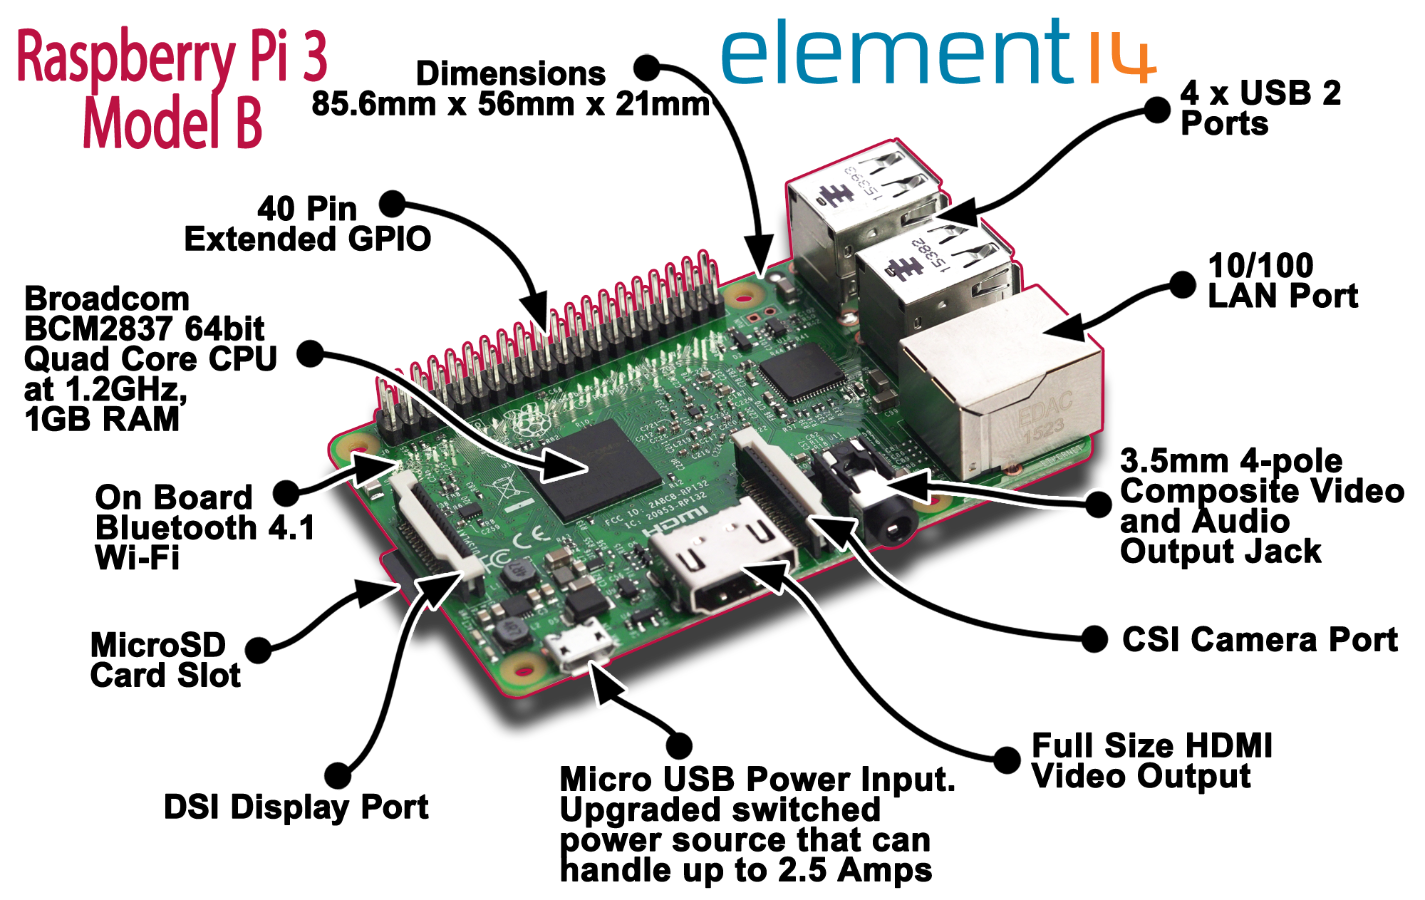
\includegraphics[width=0.9\linewidth]{imagenes/Pi3+Breakout+Feb+29+2016.png}
	\caption{Especificaciones técnicas y conexiones físicas de la \textit{Raspberry Pi 3 modelo B} - \textit{Element 14} \cite{raspberry-pi-3-model-b-specs}}
	\label{rpi3-b-specs}
\end{figure}

\section{Desarrollo del sistema operativo}

Una vez que hemos hablado sobre placas reducidas y microcomputadores, definamos los paquetes de soporte necesarios (\textbf{\textit{BSP, Board Support Packages}}), ya que nos cruzaremos con este término cada vez que queramos desarrollar un sistema operativo basado en una placa específica; y mejor aún, nos permitirá portar un sistema prácticamente idéntico de una arquitectura a otra.\\

Según \textit{Tammy Noergaard} y \textit{Jean Labrosse} \cite{embedded-software-know-it-all-bsp}, se trata de un componente opcional integrado por el proveedor en el sistema operativo, y cuyo propósito principal es proveer de una capa de abstracción entre el sistema operativo y los controladores de dispositivo genéricos.\\

Un \textit{BSP} provee de llamadas al sistema a las capas superiores (las de software) para abstraerlas de los modos del procesador, las tablas de interrupciones y el control de registros.\\

Estos paquetes de soporte nos facilitarán enormemente el desarrollo de un sistema operativo para una placa específica como la \textit{Raspberry Pi}. En el caso de que una empresa quisiera desarrollar todos los aspectos de un sistema empotrado, incluyendo el apartado hardware, los ingenieros electrónicos harían bien en facilitar un \textit{BSP} a los desarrolladores de aplicaciones embebidas que trabajen en el proyecto; dada la facilidad y el ahorro de tiempo que supondrían.\\

\subsection{Elección de la infraestructura software}

En este punto, dejé de tener influencia por parte de la empresa, ya que era el único con conocimientos profundos de \textit{Linux} y era el responsable de valorar las alternativas. No eran demasiadas, ya que las únicas interesantes que encontré fueron \textit{el Proyecto Yocto} (\textit{derivado de Open Embedded}), del que ya venimos hablando; y \textit{Buildroot}.\\

La premisa de ambas herramientas es la de construir un sistema \textit{Linux} completamente personalizado, incluyendo \textit{bootloader} (esto es, la parte de la placa que carga el sistema operativo), \textit{toolchain} (herramientas para el desarrollo de programas sobre la placa) y \textit{kernel} (núcleo \textit{Linux} del sistema operativo). Además comparten la característica de compilar todo íntegramente desde el código fuente público de cada uno de los módulos, utilizando (si es necesario) \textbf{compilación cruzada}. Esto permite compilar programas y módulos en una arquitectura diferente a la del dispositivo final (por ejemplo, el desarrollo de una aplicación embebida podría realizarse en un ordenador \textit{x86\_64} para ejecutarse en una \textit{Raspberry Pi} con arquitectura \textit{ARM}).\\

Veamos una comparación de las dos alternativas de código abierto más grandes para este fin, comentando ventajas e inconvenientes de cada una. Nos apoyaremos en el documento que me ayudó a tomar la decisión, perteneciente a un evento producido en 2016 en el que \textit{Alexandre Belloni} y \textit{Thomas Petazzoni} mostraban las características, potestades y debilidades de cada proyecto \cite{yocto-vs-buildroot-event}:

\begin{figure}[H]
	\centering
	
\includegraphics[width=0.6\linewidth]{imagenes/buildroot_rpi_yocto_logos.jpg}
	\caption{Logos de \textit{Buildroot},\textit{ Raspberry Pi} y \textit{the Yocto Project}} - \cite{imagen-buildroot-rpi-yocto}
	\label{rpi-buildroot-vs-yocto}
\end{figure}

\subsection{Buildroot}

\begin{itemize}
	\item Se enfoca principalmente a la \textbf{simplicidad}, por lo que aunque es sencillo de usar y tiene una curva de aprendizaje no muy grande, no es demasiado extensible.
	\item Se basa en herramientas muy tradicionales como lo son  \textbf{\textit{Kconfig}} (lenguaje de programación para configuración del kernel \cite{kconfig}) y \textbf{\textit{make}} (conocidísima herramienta de compilación por lotes de proyectos \cite{make-tool}).
	\item Muestra una forma muy fácil de configurar el sistema deseado, pues basta con ejecutar \texttt{make menuconfig} para tener una interfaz en modo terminal con la que marcar/desmarcar opciones de paquetes que deberán ser instalados. Esta configuración completa se guarda al completo en un archivo \textit{defconfig}. Finalmente, con lanzar \texttt{make} ya da comienzo la compilación del sistema final.
	\item Si se quiere generar el mismo sistema para arquitecturas diferentes, como por ejemplo una versión de producción para la \textit{Raspberry Pi} y otra de pruebas para virtualizar con \textit{QEMU}, es necesario disponer de dos carpetas de compilación separadas.
	\item Concentra todo el catálogo de paquetes en un solo repositorio oficial, lo que permite una mayor supervisión del código incluido por parte de los expertos pero limita la extensibilidad del proyecto.
\end{itemize}

\subsection{Yocto Project}

\begin{itemize}
	\item Deriva del proyecto \textit{Open Embedded}, que a priori permitía elaborar distribuciones de \textit{Linux} propias solamente para la arquitectura \textit{QEMU} (orientada a virtualización). Sin embargo, una vez conformado el proyecto \textit{Yocto}, da soporte a la mayoría de máquinas.
	\item En cuanto a lenguajes, se basa en \textit{Bitbake} y \textit{Python}. Requiere una curva de aprendizaje mayor y la configuración, que se realiza cómodamente con un editor de texto, es algo más compleja. Sin embargo, permite una mayor libertad al usuario para desarrollar módulos independientes de su interés.
	\item Provee de las dependencias del núcleo pero permite extender funcionalidades, máquinas y código a través de \textbf{\textit{layers}} (entendido en español como \textit{``capas''}). La lista de \textit{layers} puesta a disposición del proyecto se encuentra en \cite{yocto-layers-list}.
	\item Permite crear \textit{layers} independientes para las modificaciones aisladas de cada usuario (de hecho, esta es la forma idónea y más transparente de trabajar con customización de sistemas en Yocto, como aconsejan en el manual \cite{yocto-manual-own-distro}).
	\item Es un proyecto independiente dirigido por la comunidad, pero agrupa a muchos colaboradores de empresas y fabricantes como \textit{Samsung}, \textit{Atmel}, \textit{Raspberry Pi}, \textit{Freescale}, \textit{Asus} y un largo etcétera, que ponen a disposición de los usuarios paquetes \textit{BSPs} de sus placas.
\end{itemize}

Vistas las diferencias, podemos constatar que \textit{Yocto Project} se trata de una alternativa más férrea y profesional, que cuenta con una comunidad numerosa compuesta de gente influyente y activa en el sector. Por si esto fuera poco, tras haber probado ambas alternativas durante un tiempo, es muy notable la flexibilidad que comporta, mientras que su ``rival'' limita mucho a la hora de dar rienda suelta a la creatividad (o mejor dicho, las necesidades) del usuario. Por tanto, el proyecto habrá sido basado en esta alternativa.

\section{Gestor de actualizaciones}

Otra parte importante del proyecto reside en \textbf{las actualizaciones}. Para ser vendido a nivel internacional, \textit{DYNAsystem} necesita disponer de una herramienta de mejora de su software así como de depuración de posibles errores. Además, dichas actualizaciones han de verificar ciertos requisitos de seguridad, asegurando que una instalación fallida no dejaría incomunicada a la máquina o al usuario sin poder trabajar con ella cuando lo quisiese. Por esto, buscaremos especialmente un sistema de actualizaciones con \textbf{soporte para \textit{rollback}}, herramienta que detecta cuando una actualización ha sido realizada correctamente y cuando no, volviendo a la versión anterior para que el dispositivo siga en funcionamiento.\\

Una vez decidida la implementación de un sistema embebido basado en \textit{Yocto} sobre la \textit{Raspberry Pi}, ``tan solo'' es necesario encontrar un gestor de actualizaciones que soporte ambas tecnologías. En la referencia \cite{yocto-system-update} tenemos una lista de las plataformas disponibles en los \textit{layers} antes mencionados. Veamos un resumen de cada una de las alternativas:

\begin{itemize}
	\item \textbf{\textit{swupd}}: distribuye el sistema operativo en (al menos) una sola partición, seleccionando los ficheros que deben ser actualizados. Su código está alojado en el layer \textbf{\textit{meta-swupd}} \cite{meta-swupd} y, según dicha \textit{wiki} del proyecto, resulta ser un sistema bastante fiable y seguro para actualizaciones frecuentes. Sin embargo, no dispone de un sistema por defecto de recuperación frente a errores, lo que le resta peso como alternativa.
	\item \textbf{\textit{sbabic's swupdate}}: también es flexible en cuanto a particionamiento y sus módulos están alojados en \textbf{\textit{meta-swupdate}} \cite{meta-swupdate}. Exige imágenes cifradas y transmitidas mediante \textit{HTTPS}, lo que le transfiere seguridad. Lamentablemente, también necesita de trabajo extra para instalar un sistema de \textit{roll-back}.
	\item \textbf{\textit{Mender}}: se basa en un esquema de cuatro particiones (arranque, sistema de ficheros \#1, sistema de ficheros \#2 y partición de datos persistente); siendo \#1 y \#2 dos sistemas de ficheros inicialmente iguales pero que se irán alternando con la sucesión de actualizaciones. Es decir, cuando una de ellas esté activa y se detecte una actualización, ésta será instalada en la partición en desuso, que se marcará como ``activa'' para el siguiente arranque del dispositivo. También funciona sobre \textit{HTTPS} y permite cifrado de imágenes. Afortunadamente, \textbf{posee soporte para \textit{roll-back}}, por lo que si al iniciar desde la segunda partición no consigue dar parte al servidor de que se ha actualizado, considera fallida la actualización y se vuelve a activar la partición previa. El layer dedicado es \textbf{meta-mender} \cite{meta-mender}, su código es estable y está bajo desarrollo activo.
	\item \textbf{\textit{OSTree}}: al igual que \textit{Mender}, se trata de otra alternativa adecuada para el proyecto; ya que aún siendo flexible en cuanto a particionamiento, contiene soporte de recuperación en cuanto a actualizaciones fallidas, sea por caídas de conexión o de corriente eléctrica. Tiene una base de usuarios significativa y un ciclo de desarrollo rápido en su capa \textbf{\textit{meta-updater}} \cite{meta-updater}.
	\item \textbf{\textit{RAUC}}: también flexible en cuanto a bloques de dispositivo, exige que las imágenes comprimidas viajen firmadas con el protocolo \textit{X.509}. Tiene disponible la función de \textit{rollback} siempre y cuando el \textit{bootloader} integrado la soporte. Sus módulos están disponibles en \textbf{meta-rauc} \cite{meta-rauc}.
\end{itemize}

Una vez vistas las alternativas, constatamos que las más interesantes son las tres últimas, dado que permiten recuperación del sistema en caso de error o actualización fallida. Sin embargo, la diferencia vendrá dada por el modo de centralización de las diferentes versiones, pudiendo ser repositorios de código aislado o servidores propios debidamente administrados.\\

Con respecto a esto, la empresa desarrolladora de \textit{Mender} (\textit{Northern Tech} \cite{northern-tech}) ofrece una alternativa de pago más que interesante: \textbf{\textit{Hosted Mender}}, que consiste en la puesta a punto y el mantenimiento de un servidor donde alojar las actualizaciones, y con el que comunican cada uno de los dispositivos clientes. Partiendo de esto, el desarrollador solo tiene que preocuparse de integrar el sistema operativo con la comunicación al servidor, así como de ir subiendo las imágenes cifradas a dicho servidor y finalmente eligiendo en el portal web los dispositivos a los que se quiere desplegar la imagen actualizada. Esta alternativa permite a la empresa ahorrar el tiempo de un ingeniero dedicado a la administración del servidor, y por lo tanto el coste que ello supone.\\

Por otro lado, en \textbf{\textit{meta-mender}} \cite{meta-mender} disponemos de la lista de paquetes y utilidades necesarias para dicha integración, mientras que en la documentación \cite{docs-mender} encontramos los pasos requeridos para ello; que utilicé para realizar las pruebas con este software. Dado que \textit{Hosted Mender} permitía una fase beta gratuita de pruebas, dediqué tiempo a experimentar con este software, intercambiando correos con los responsables cuando me surgía alguna duda al respecto, quienes me respondieron y ayudaron de buena gana. Finalmente, decidí optar por esta alternativa, ya que cumplía todas las expectativas y, tras comentarlo con mi empresa, decidimos que era la mejor opción en cuanto a resultados, tiempo y dinero.

\newpage
